\documentclass{beamer}
\usetheme{Madrid}
\usepackage{graphicx}
\usepackage{booktabs}
\usepackage{amsmath, amsfonts}
\usepackage{tikz}
\usepackage{adjustbox}
\usetikzlibrary{bayesnet}

\setbeamertemplate{navigation symbols}{}

% Short title for footer display
\title[Zillow Housing Forecast]{The Cost of Living: A Zillow Housing Forecast}
\author[Beal, Eddington, Vines]{Patrick Beal \\ Tiara Eddington \\ Madelyn Vines}
\date{Math 404 Data Project Presentation}

\begin{document}

% Madi
\frame{\titlepage} 

% Madi
\begin{frame}{Motivation \& Goals}
  \begin{itemize}%[<+->]
    \item Housing prices shape wealth, policy, and investment.
    \item We aim to:
    \begin{itemize}%[<+->]
      \item Identify similar housing markets (clustering).
      \item Forecast housing prices using multiple models.
      \item Identify correlations between housing markets and demographic features.
    \end{itemize}
    \item Focus on interpretable and regional trends.
  \end{itemize}
\end{frame}

% Patrick
\begin{frame}{Data Overview} 
  \begin{itemize}%[<+->]
    \item \textbf{Zillow HPI:} State-level median home prices (monthly, 2000--2020).
    \item \textbf{CPS/IPUMS:} Demographics, income, and tax (annual, interpolated).
    \item Filtered to pre-COVID period.
  \end{itemize}
\end{frame}

% Madi
\begin{frame}{Clustering States by Price Trends} 
\begin{center}
  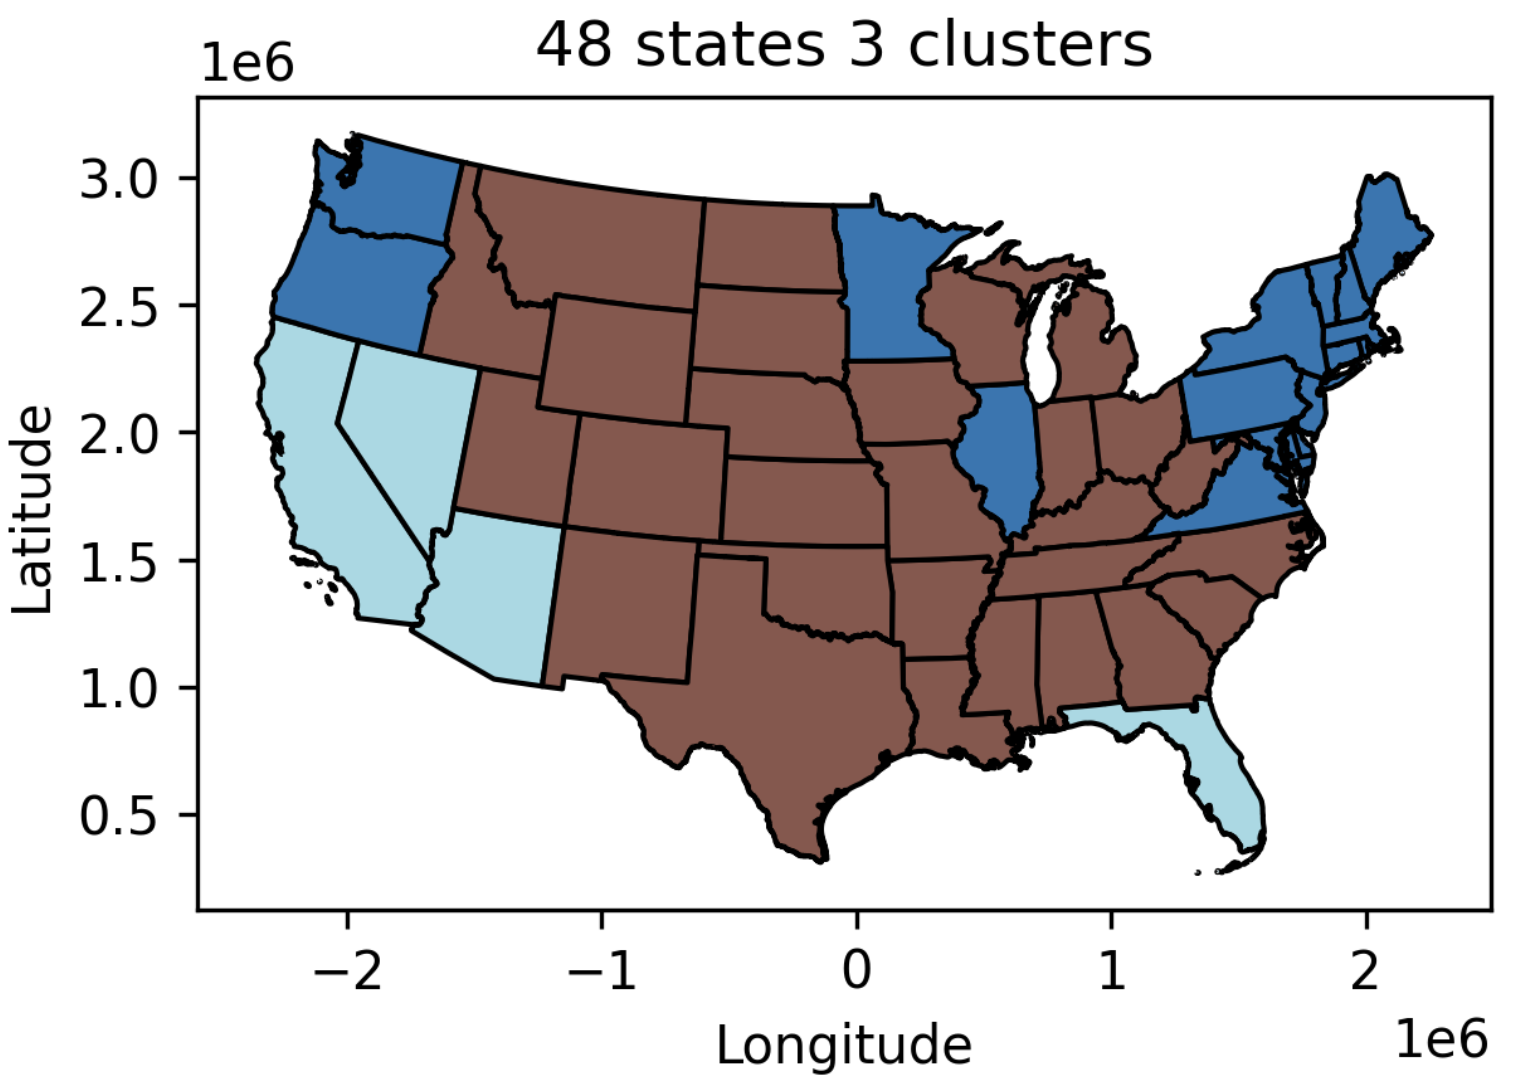
\includegraphics[width=0.4\linewidth]{figures/3clusters.png}
  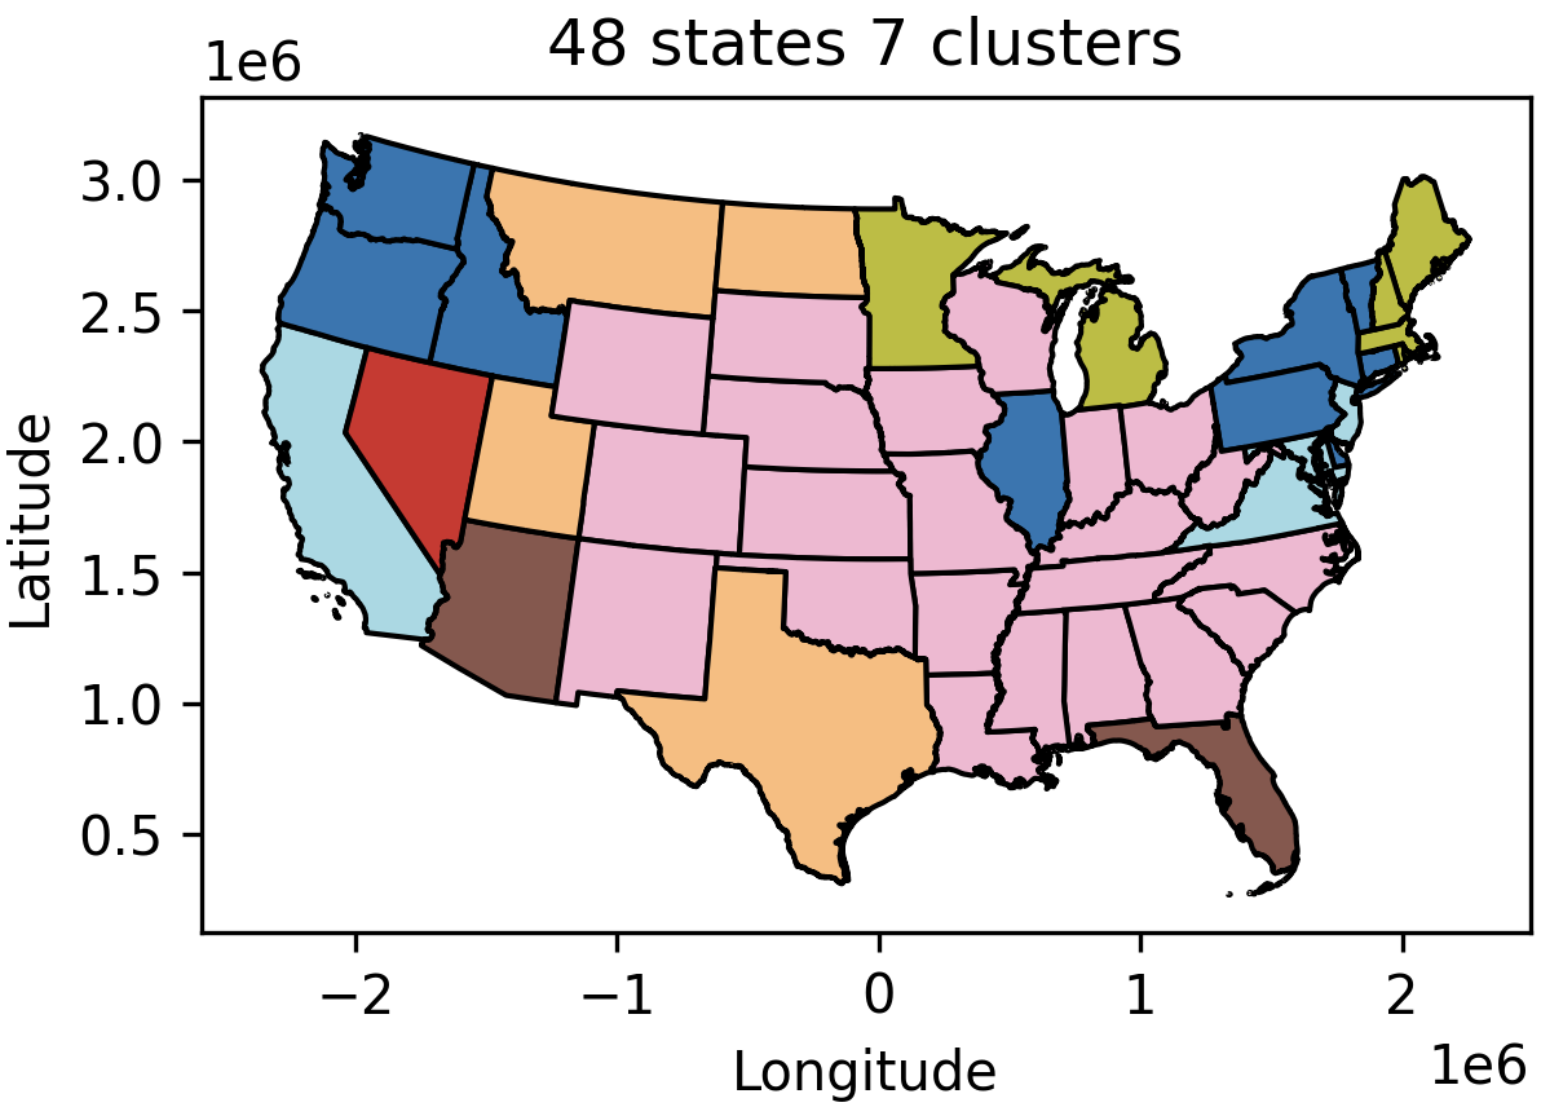
\includegraphics[width=0.4\linewidth]{figures/7clusters.png}
\end{center}
  % \pause
  \begin{itemize}%[<+->]
    \item K-means on housing price changes $\Rightarrow$ groups with similar growth.
    \item Coastal states form distinct clusters.
  \end{itemize}
\end{frame}

% Tiara
\begin{frame}{Classical Decomposition of Housing Prices} 
\begin{center}
  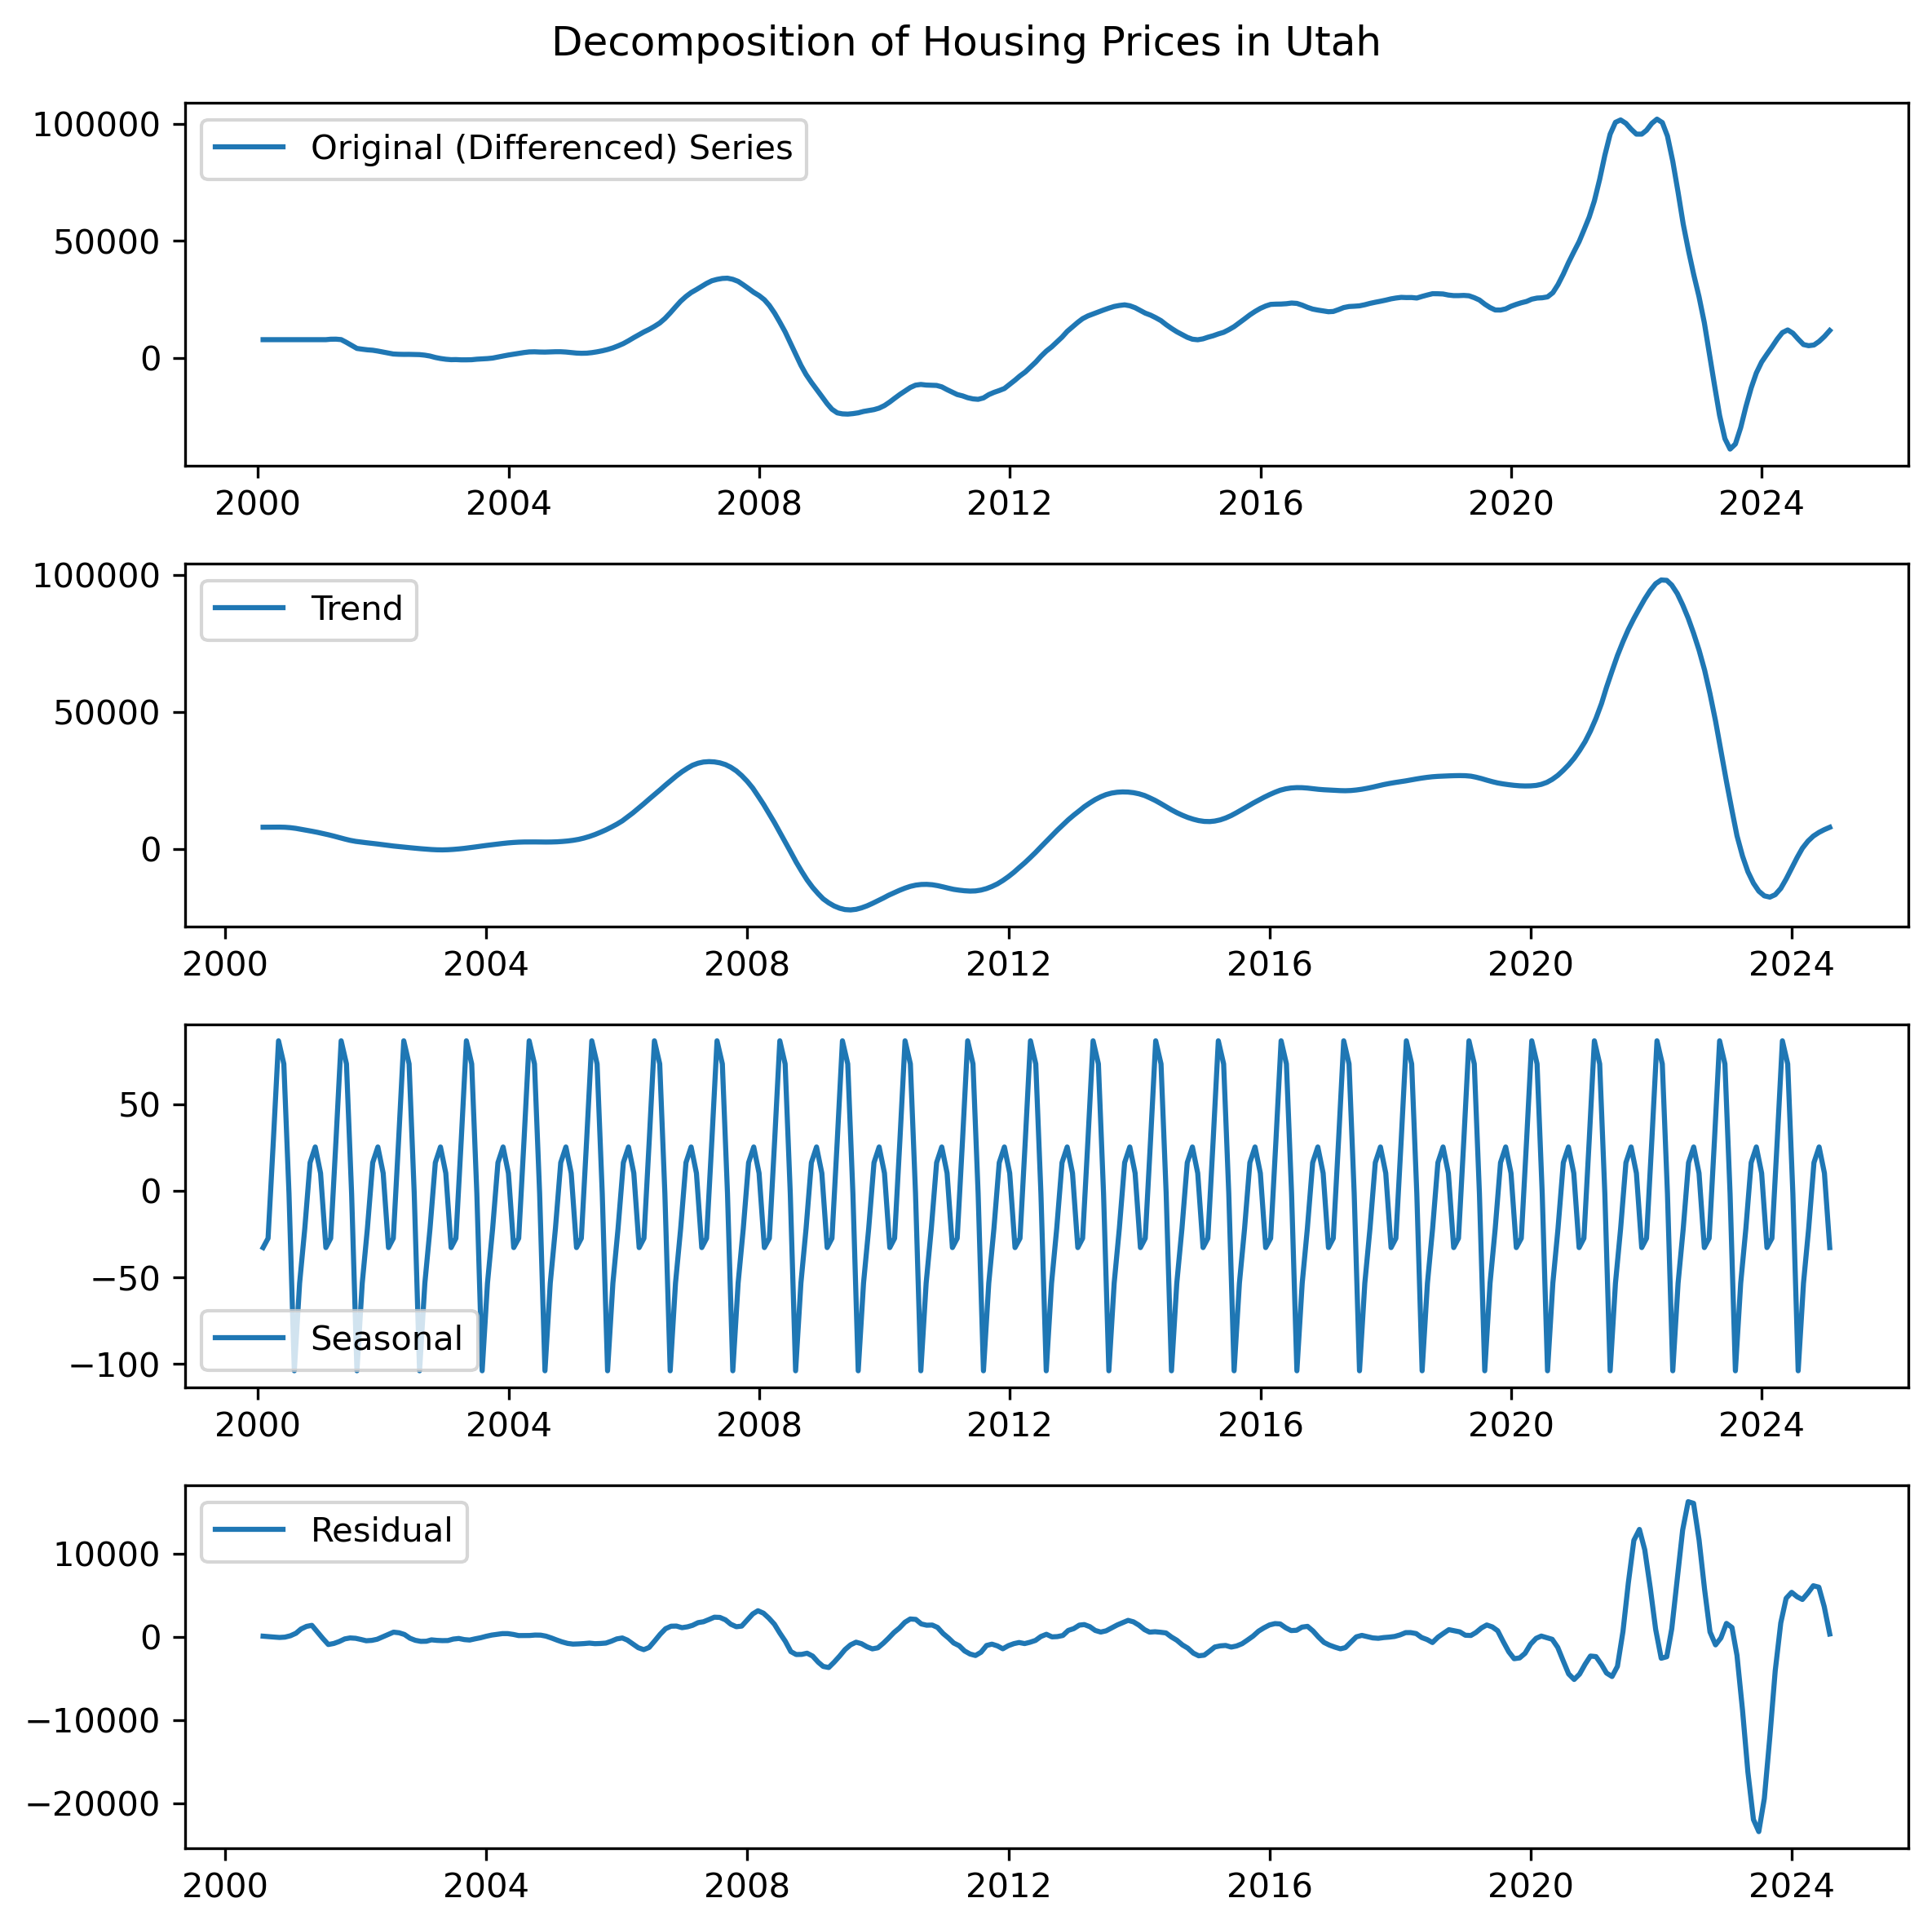
\includegraphics[width=0.45\linewidth,trim={0 3.8in 0 0.3in},clip]{figures/utah_prices.png}
  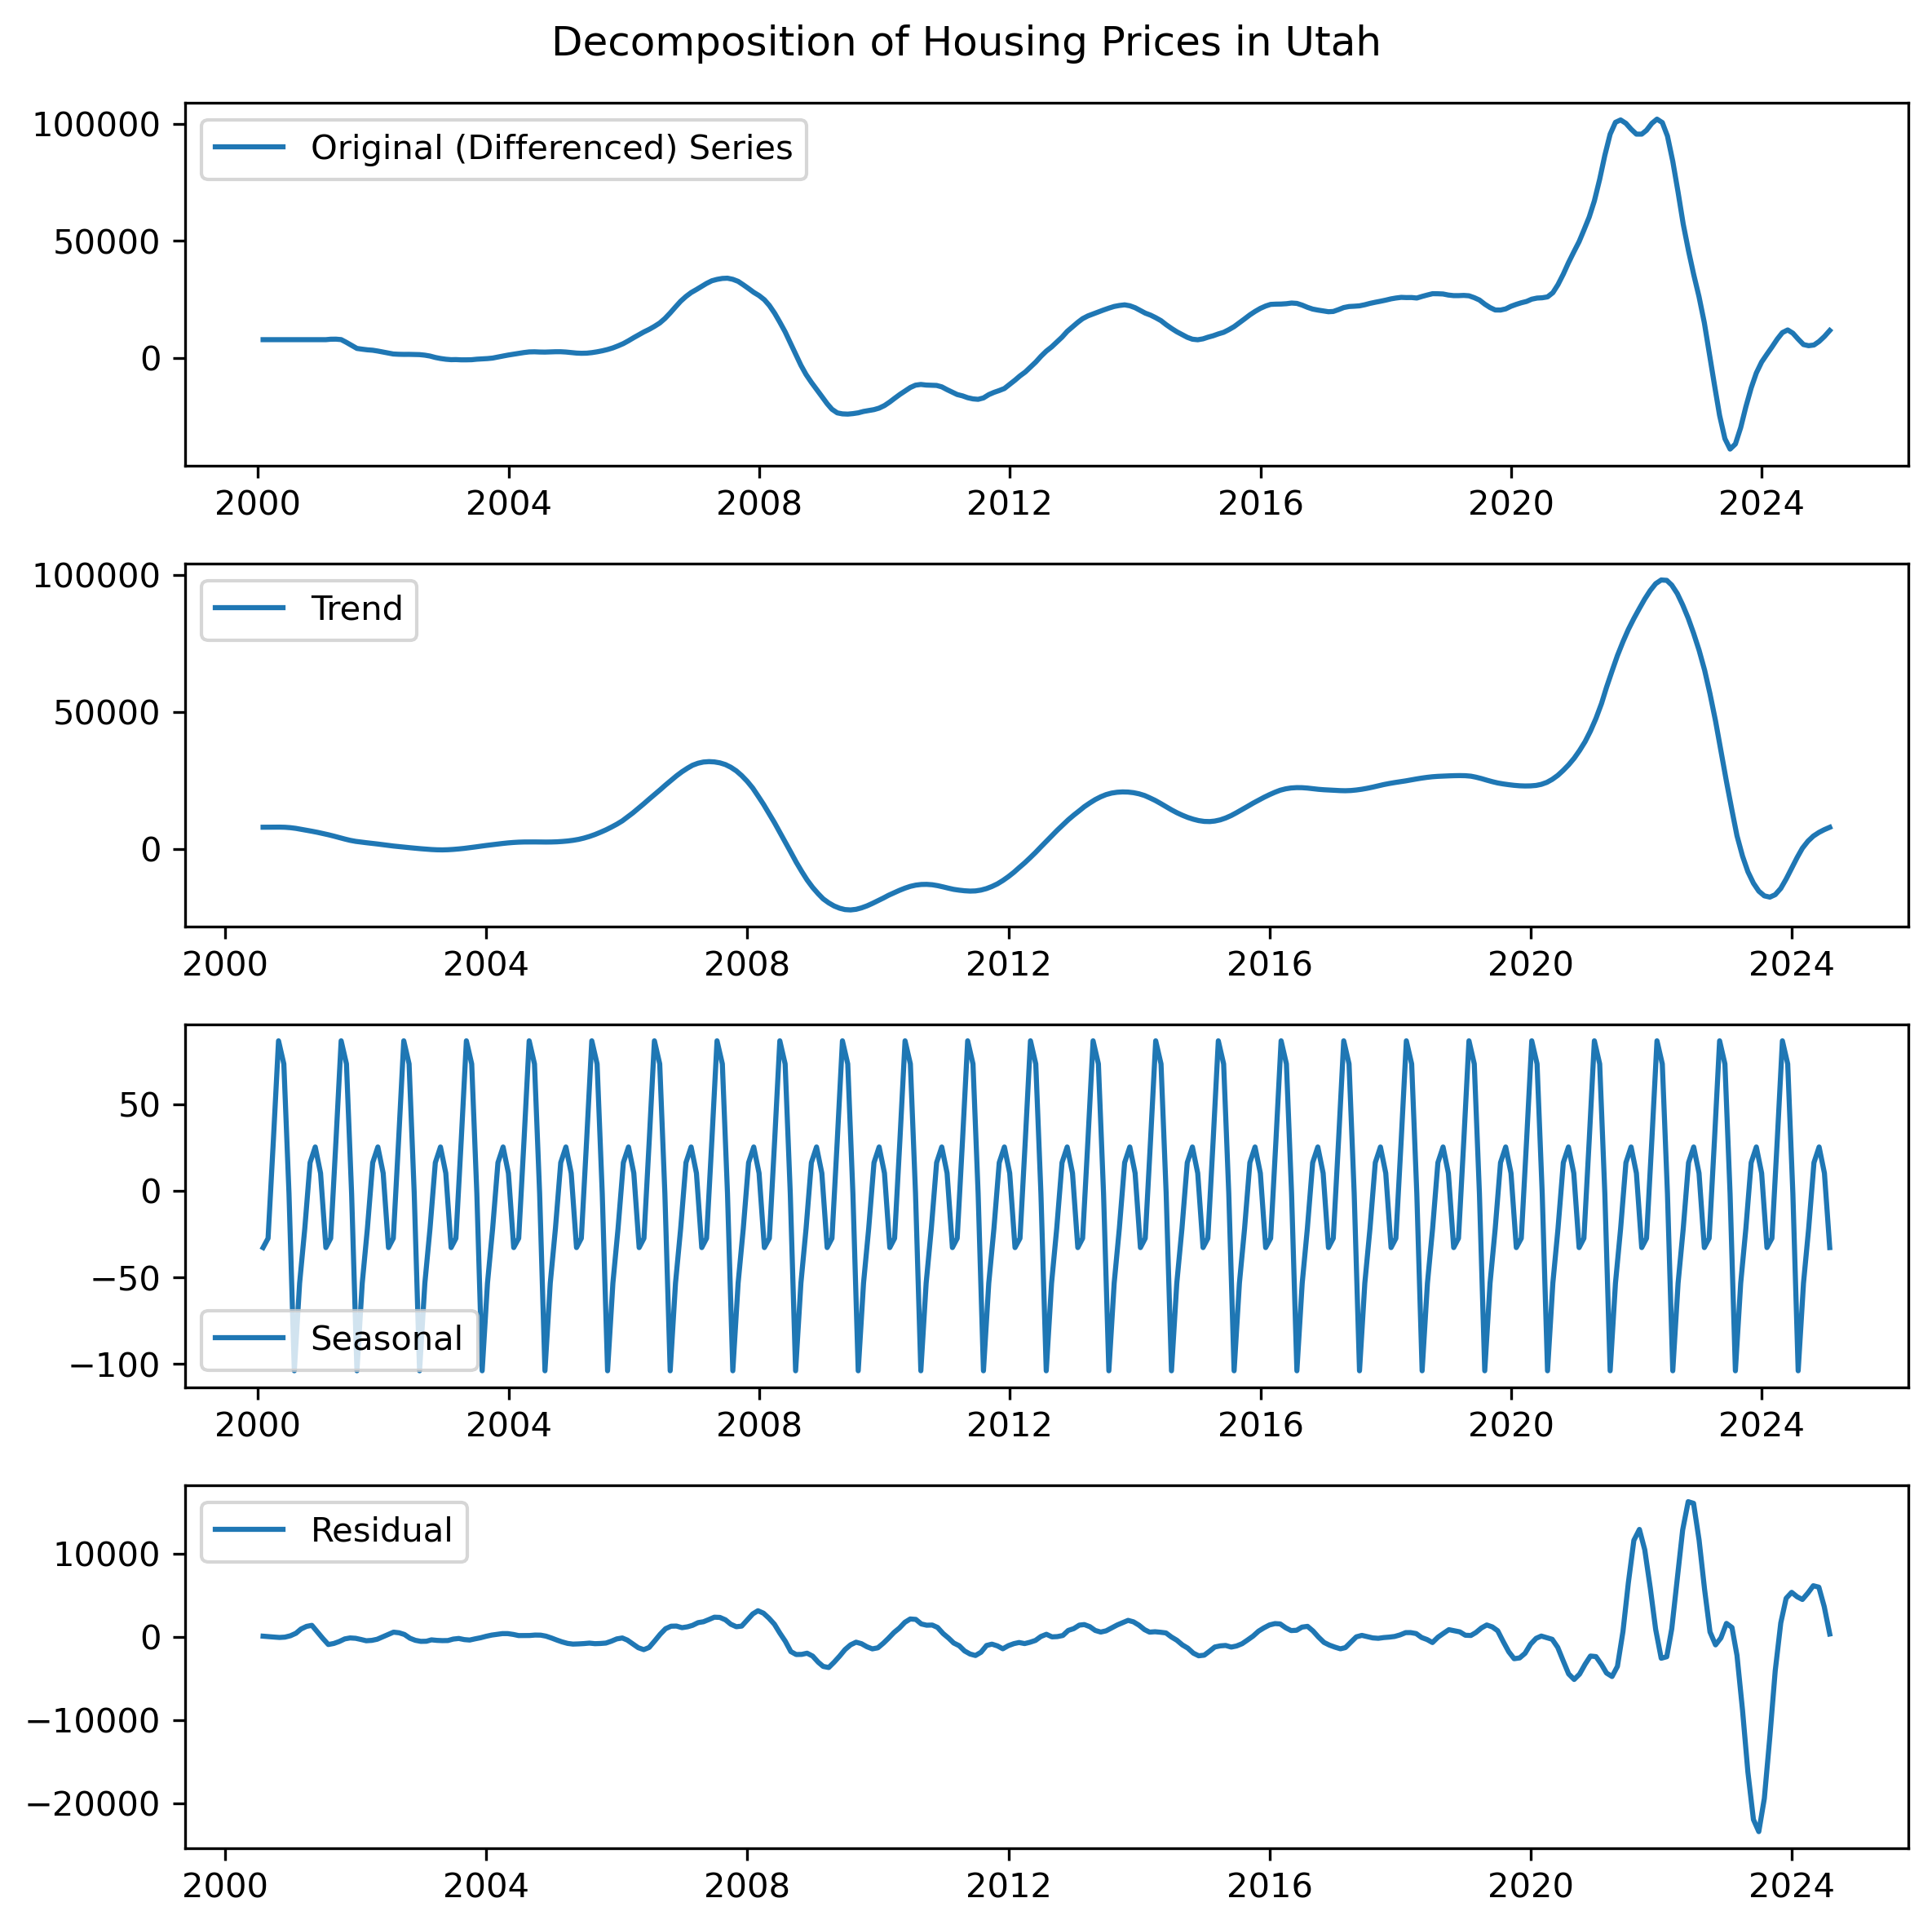
\includegraphics[width=0.45\linewidth,trim={0 0 0 4.1in},clip]{figures/utah_prices.png}
\end{center}
  % \pause
  \begin{itemize}%[<+->]
    \item Classical decomposition $\Rightarrow$ double-peaked seasonal trends.
    \item Residuals spike after 2020 $\Rightarrow$ excluded post-2020.
  \end{itemize}
\end{frame}

% Tiara
\begin{frame}{Univariate ARIMA Forecasting} 
\begin{center}
  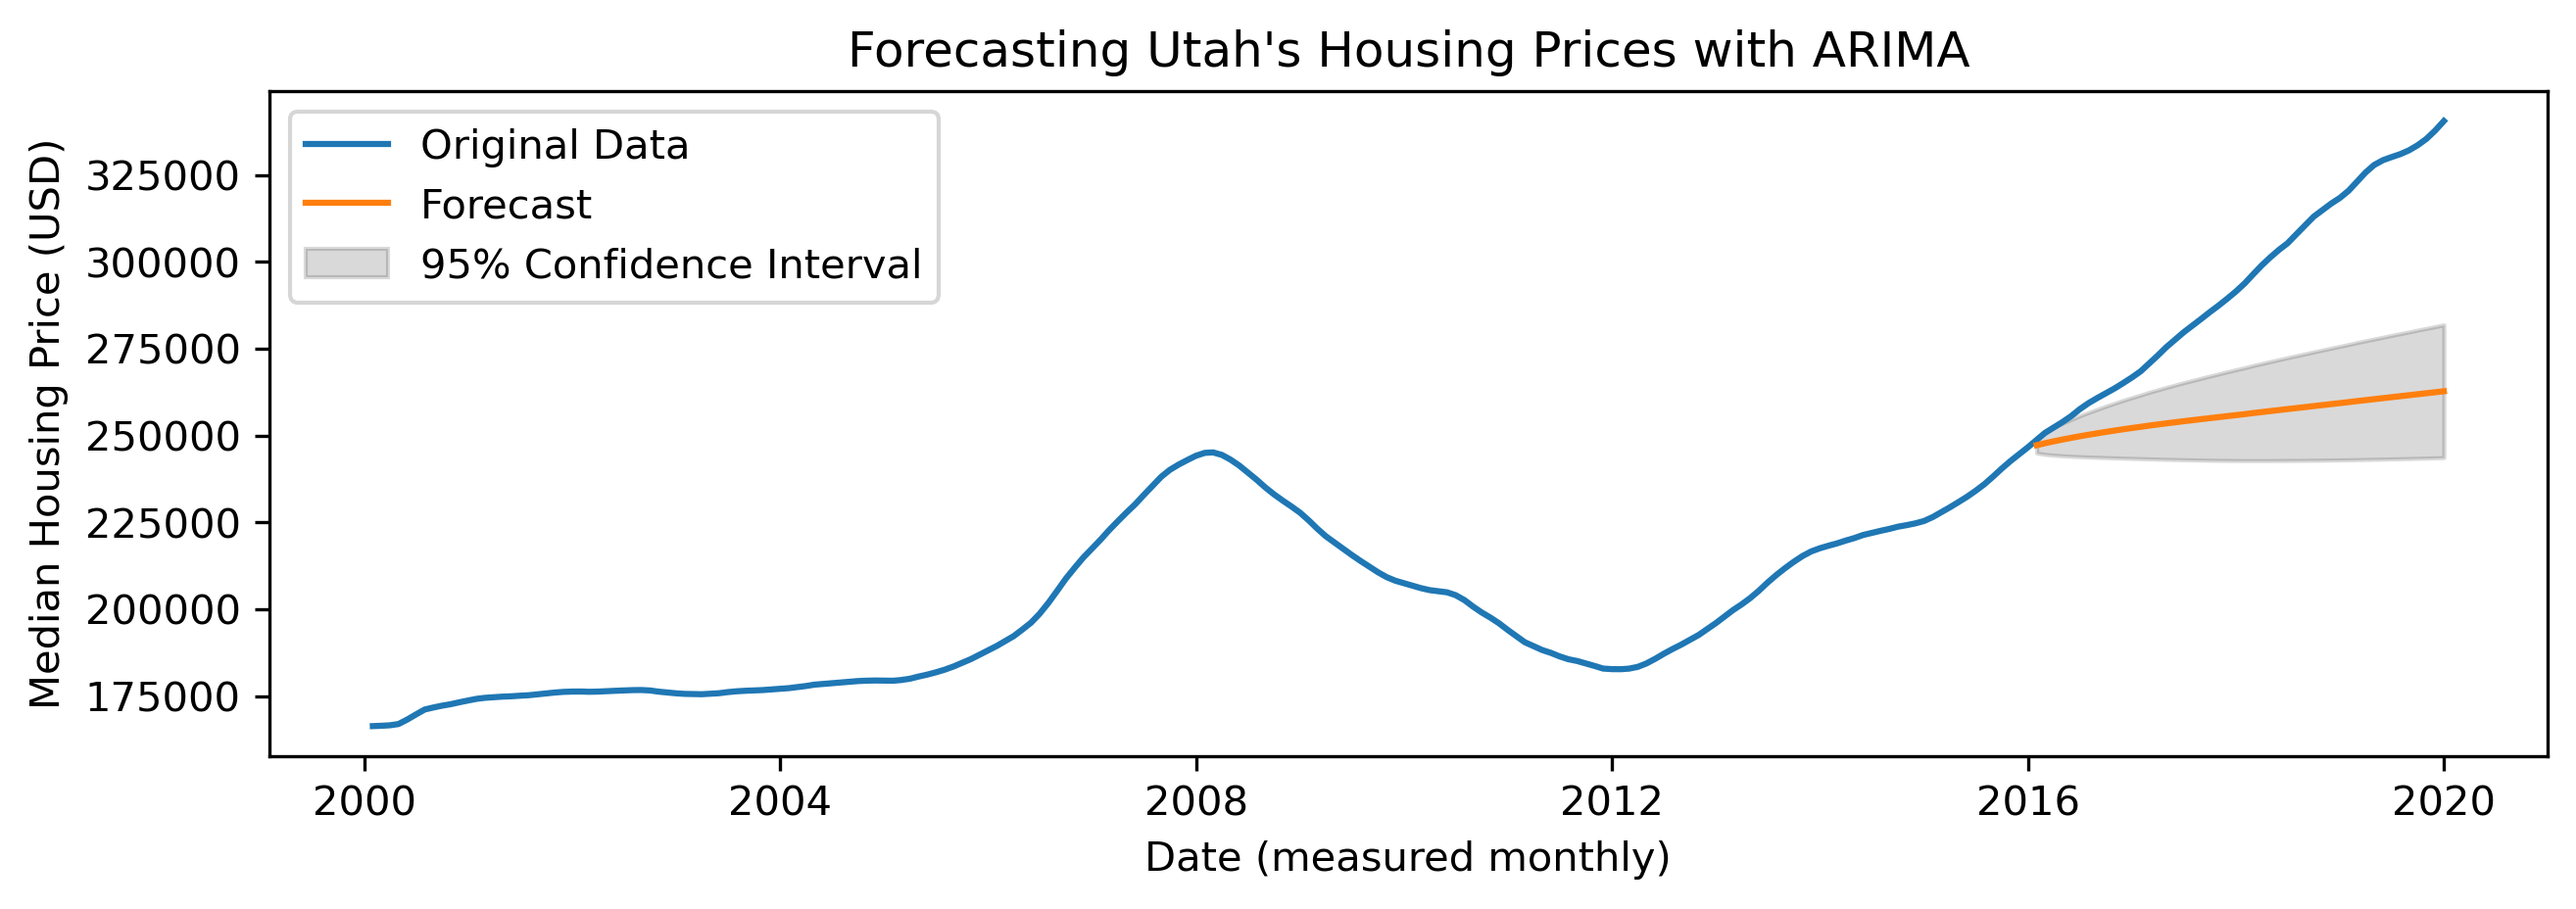
\includegraphics[width=0.75\linewidth]{figures/Utah_forecast_long.png}
\end{center}
\begin{center}
  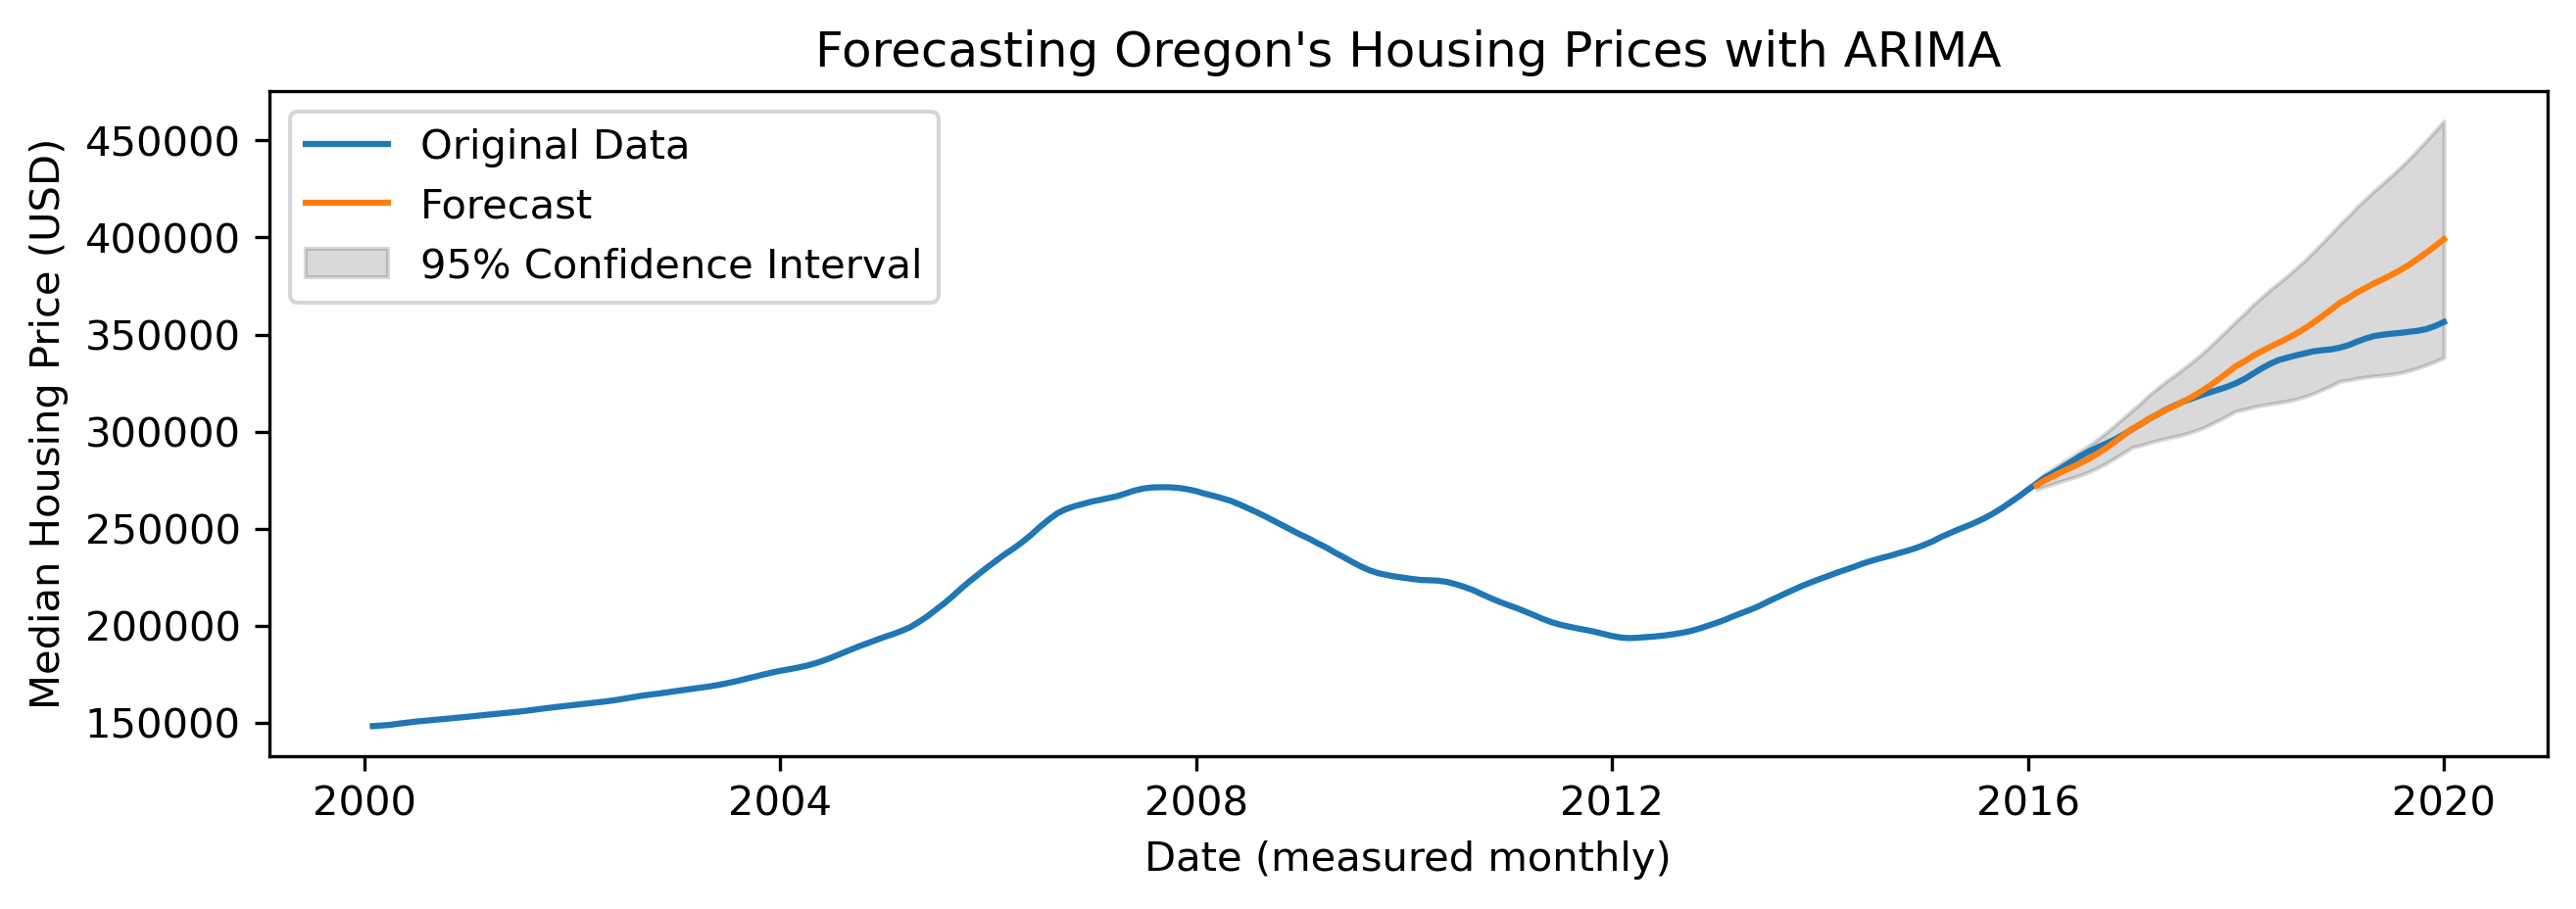
\includegraphics[width=0.75\linewidth]{figures/Oregon_forecast_long.png}
\end{center}
  % \pause
  \begin{itemize}%[<+->]
    \item Best ARIMA model: (4,1,0) -- approximately linear forecasts
    \item Limited accuracy: large confidence intervals, sensitivity to shocks
  \end{itemize}
\end{frame}

% Tiara
\begin{frame}{VARMAX Forecasting} 
  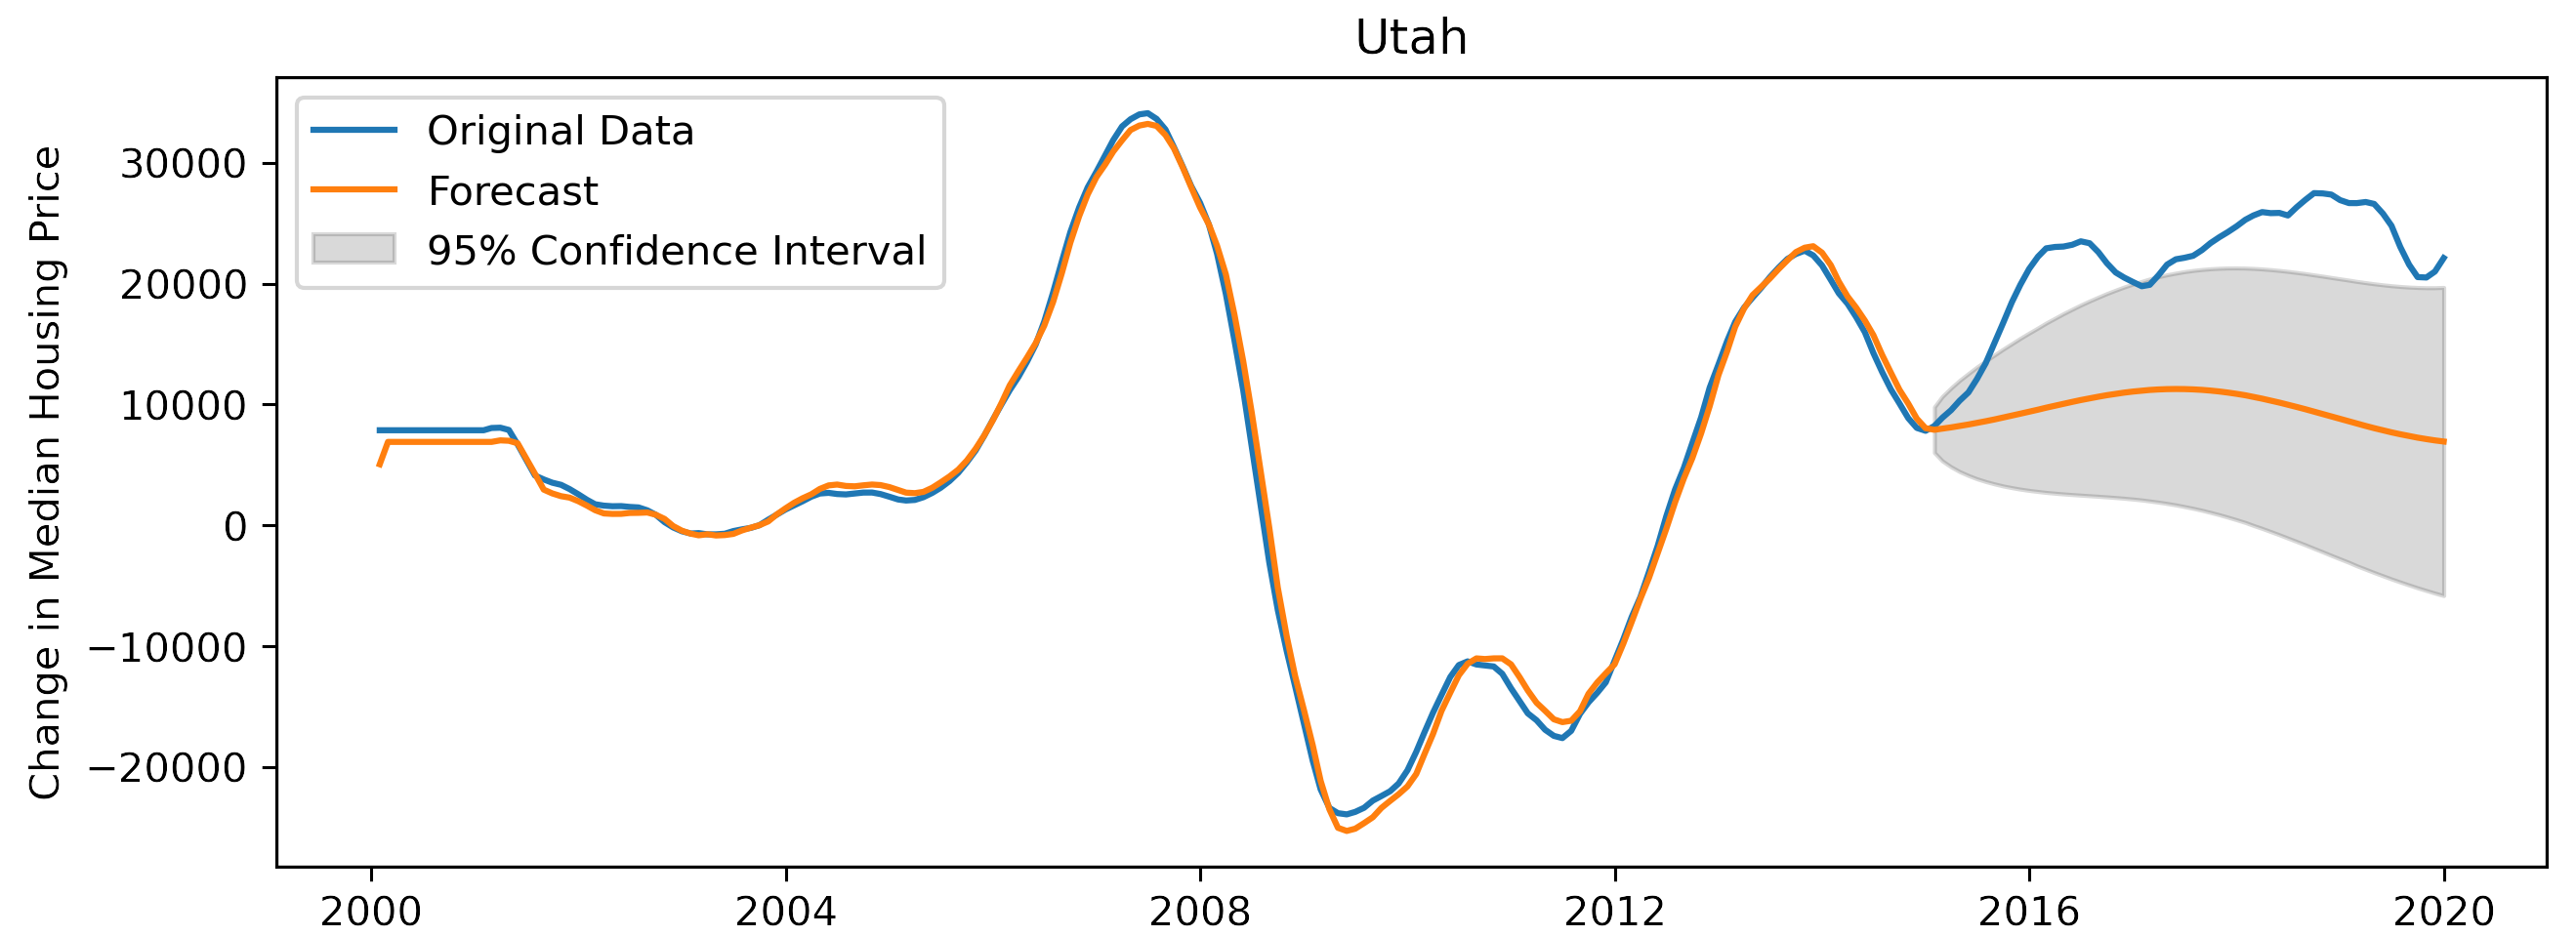
\includegraphics[width=0.9\linewidth]{figures/utah_varmax.png}
  % \pause
  \begin{itemize}%[<+->]
    \item Cluster-based VARMAX $\Rightarrow$ improved trend modeling
    \item Not applicable to states in singleton clusters
    \item Using demographic data led to convergence issues
  \end{itemize}
\end{frame}


% Patrick 
\begin{frame}{Bayesian Hierarchical Model Diagram} 
\begin{center}
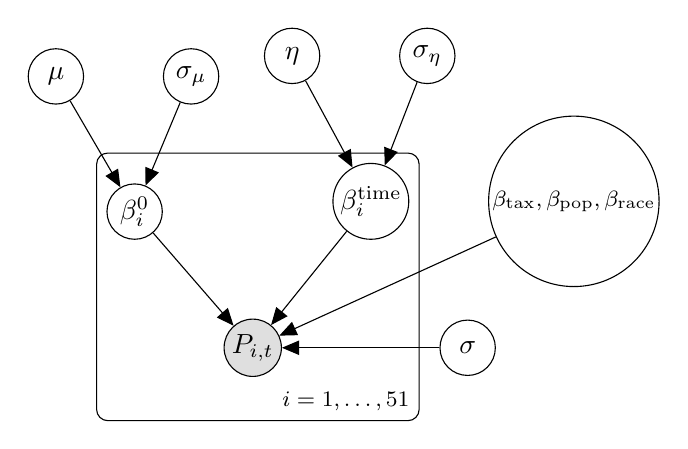
\begin{tikzpicture}

  % Observed node
  \node[obs]                      (P)   {$P_{i,t}$};

  % Latent state-level parameters
  \node[latent, above=of P, xshift=-1.5cm] (beta0i) {$\beta_i^0$};
  \node[latent, above=of P, xshift=1.5cm]  (betati) {$\beta_i^{\text{time}}$};

  % Global coefficients
  \node[latent, right=of betati] (global) {\footnotesize $\beta_{\text{tax}}, \beta_{\text{pop}}, \beta_{\text{race}}$};

  % Hyperpriors for state-level
  \node[latent, above=of beta0i, xshift=-1cm] (mu) {$\mu$};
  \node[latent, right=of mu] (sigmamu) {$\sigma_\mu$};


  \node[latent, above=of betati, xshift=-1cm] (eta) {$\eta$};
  \node[latent, right=of eta] (sigmaeta) {$\sigma_\eta$};

  % Error variance
  \node[latent, right=of P, xshift=1.0cm] (sigma) {$\sigma$};

  % Edges
  \edge {beta0i, betati, global, sigma} {P};
  \edge {mu, sigmamu} {beta0i};
  \edge {eta, sigmaeta} {betati};

  % Plates
  \plate {state} {(P)(beta0i)(betati)} {$i = 1, \dots, 51$};

\end{tikzpicture}
\end{center}
\end{frame}

% Patrick 
\begin{frame}{Bayesian Hierarchical Model Setup} 
\small
% \begin{block}{Model Equation}
Model Equation
\begin{align*}
P_{i,t} &= \beta_i^0 + \beta_i^{\text{time}} t + \beta_{tax}\, \text{tax}_i + \beta_{pop}\, \text{pop}_i + \beta_{native}\, \alpha_{native,i} \\
&\quad + \beta_{asian}\, \alpha_{asian,i} + \beta_{black}\, \alpha_{black,i} + \beta_{white}\, \alpha_{white,i} + \epsilon
\end{align*}
% \end{block}
% \pause
% \begin{block}{Prior Distributions (Examples)}
% \end{block}
% \pause
\begin{itemize}%[<+->]
  \item Captures variation across states via hierarchical priors.
  \item Standardized predictors allow coefficient comparisons.
  \item Fit using NUTS algorithm (via PyMC3).
\end{itemize}
\end{frame}

\begin{frame}{Bayesian Hierarchical Prior Distributions}
\begin{align*}
\beta_i^0 &\sim \mathcal{N}(\mu, \sigma_\mu) & \quad \beta_i^t &\sim \mathcal{N}(\eta, \sigma_\eta) \\
\mu &\sim \mathcal N (200000, 100000) & \quad \eta &\sim \mathcal N (1000, 1000) \\
\sigma_{\mu} &\sim \text{Exp}\left(\frac{1}{50000}\right) & \quad \sigma_{\eta} &\sim \text{Exp}\left(\frac{1}{5000}\right) \\
\beta_{tax} &\sim \mathcal{N}(0, 20) & \quad \beta_{pop} &\sim \mathcal{N}(0, 1) \\
\beta_{race} &\sim \mathcal{N}(0, 10000) & \quad \epsilon &\sim \mathcal N (0, \sigma) \\
\sigma &\sim \text{HalfCauchy}(100)
\end{align*}
\end{frame}


% Patrick 
\begin{frame}{Bayesian Hierarchical Modeling} 
  \includegraphics[width=0.9\linewidth,trim={0 22in 0 0in},clip]{figures/trace_plot.png}
  % \pause
  \begin{itemize}%[<+->]
    \item State-level intercepts/slopes + global covariates.
    \item Accounts for uncertainty and data imbalance.
  \end{itemize}
\end{frame}

% Patrick

% \begin{frame}{State-level Housing Price Growth}
% 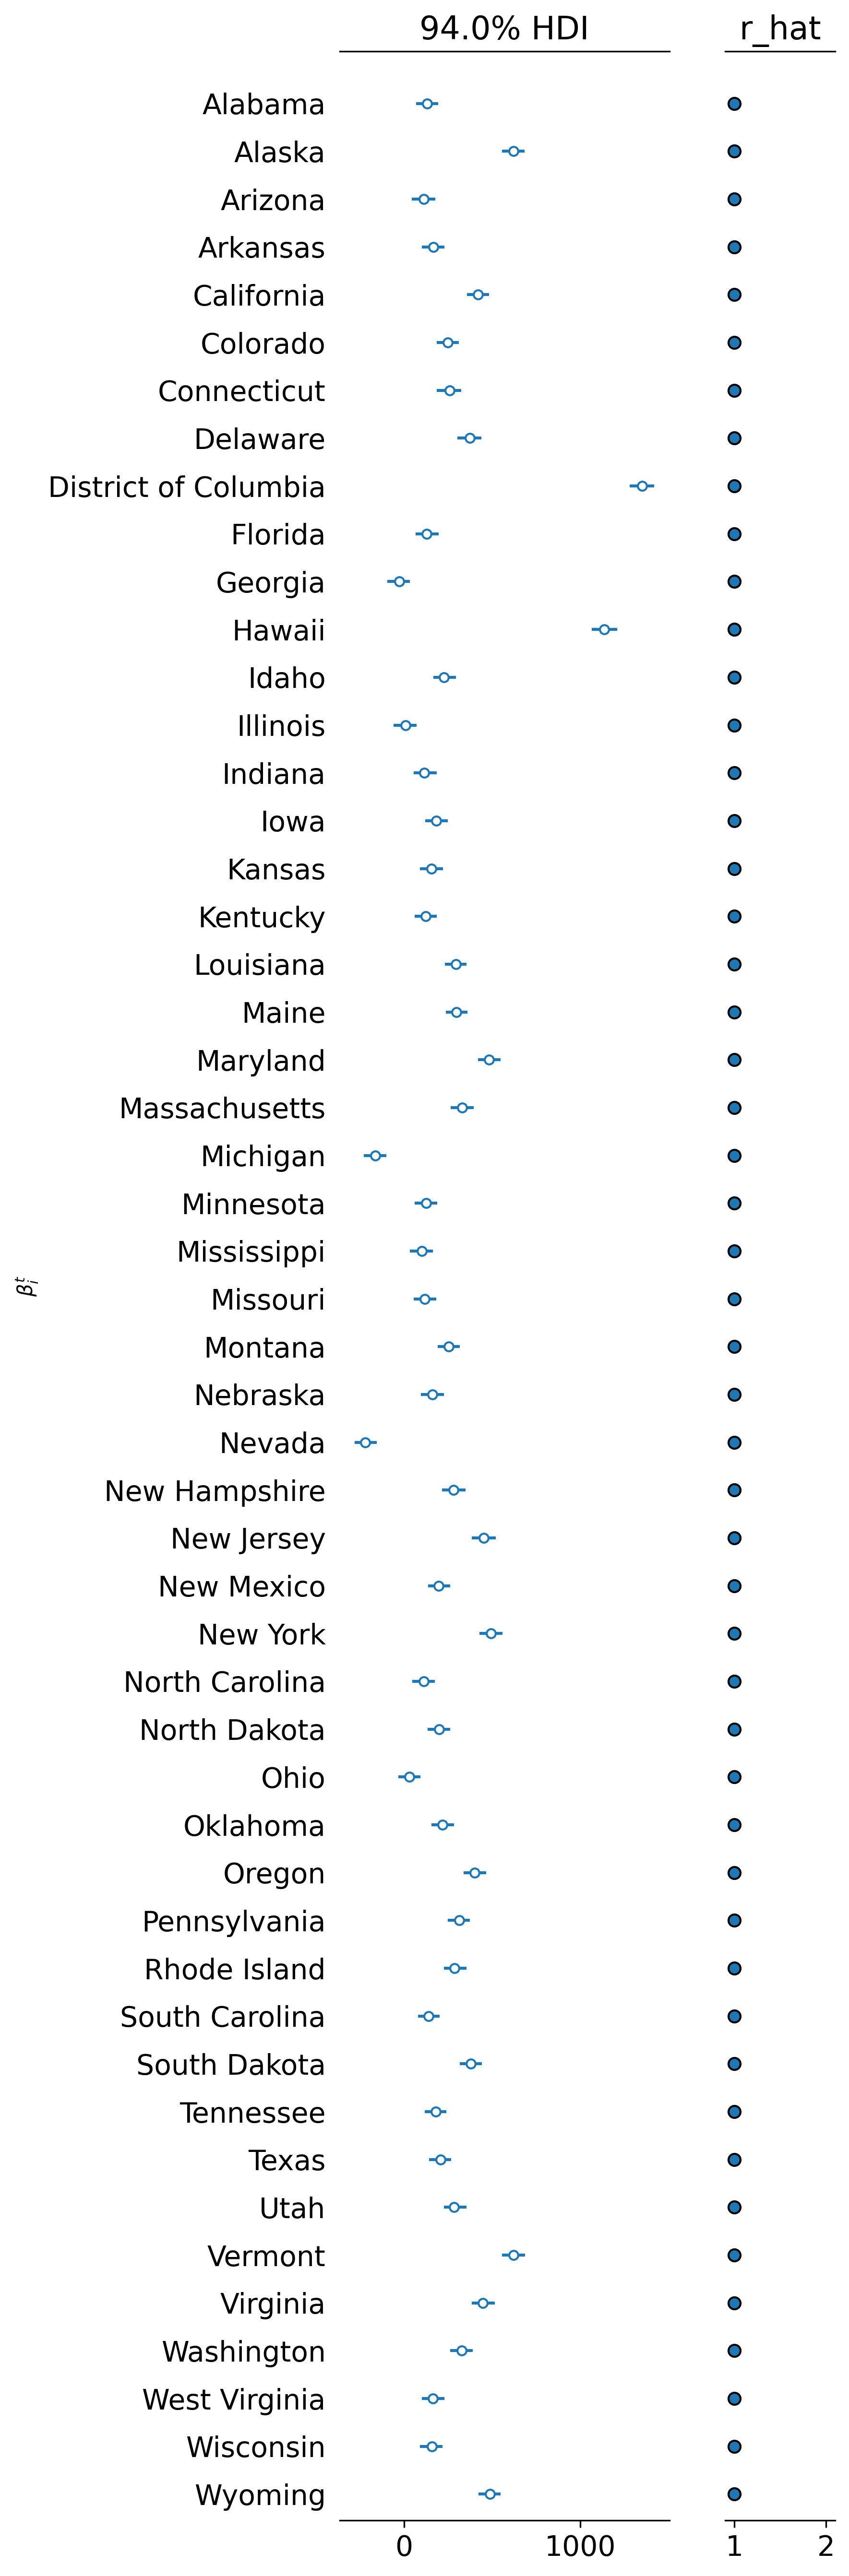
\includegraphics[height=\linewidth,angle=90]{figures/slope_forest.png}
% \end{frame}

% \begin{frame}{State-level Housing Price Intercept}
% 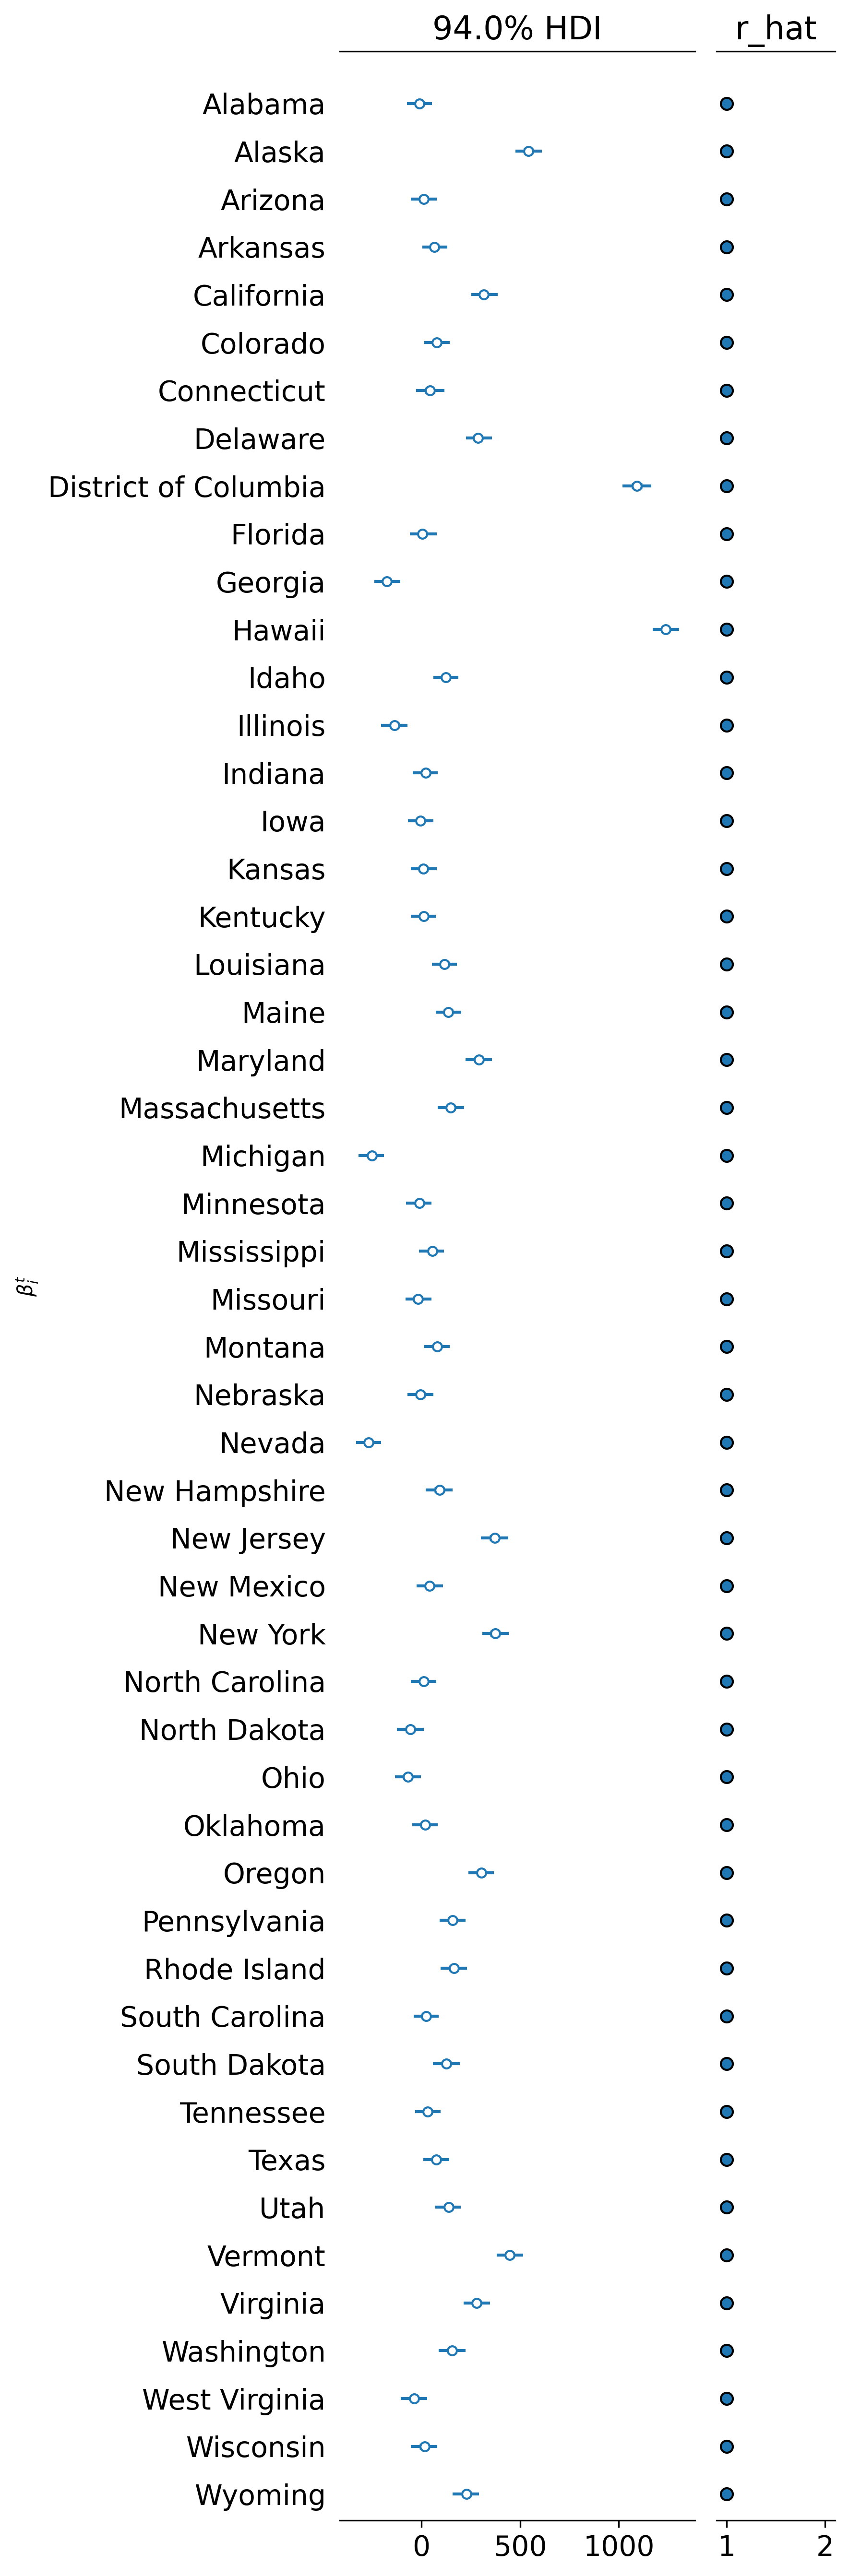
\includegraphics[height=\linewidth,angle=90]{figures/forest_plot.png}
% \end{frame}

% Tiara
\begin{frame}{Key Findings} 
  \begin{itemize}%[<+->]
    \item Central states show more homogeneous trends.
    \item ARIMA and VARMAX useful, but limited by volatility.
    \item Bayesian model provides interpretable insights:
    \begin{itemize}%[<+->]
      \item Native/Asian/White proportion $\Rightarrow$ lower prices.
      \item Black proportion $\Rightarrow$ rising prices.
    \end{itemize}
  \end{itemize}
\end{frame}

\begin{frame}{Ethical Considerations} % Madi
  \begin{itemize}%[<+->]
    \item Demographics \textbf{should not} guide individual decisions.
    \item Models risk perpetuating bias.
    \item Better use: \textit{Policy insights and funding allocation}.
  \end{itemize}
\end{frame}


% Patrick
\begin{frame}{Conclusion} 
  \begin{itemize}%[<+->]
    \item Forecasting housing prices is difficult due to shocks.
    \item Combined methods yield the best insights.
    \item Future work: Combine Bayesian models with ARIMA/Kalman filters, use more robust economic models.
  \end{itemize}
\end{frame}

\begin{frame}{Resources}
  \begin{itemize}%[<+->]
    \item GitHub Repo: \href{https://github.com/jpatrickb/vol3_housing_project}{github.com/jpatrickb/vol3\_housing\_project}
    \item Data from Zillow + IPUMS/CPS
  \end{itemize}
\end{frame}

\begin{frame}{Questions?}
  \centering
  \Large Thank you!
\end{frame}

\end{document}
